\documentclass[a4paper]{article}
\usepackage{graphicx}
\usepackage{float}

\title{ISO/IEEE 11073-10206 - ACOM (Abstract Content Information Model)}
\author{Riccardo Cambianica}
\begin{document}
    \maketitle
    \section*{ACOM Observation class}
        ACOM Observation class (da qui in poi chiamata semplicemente "la classe") descrive un modello generico per esprimere \textbf{osservazioni} fatte dai PHD. 
        E' basato sull'oggetto metrico descritto dallo standard ISO/IEEE 11073-20601 e condivide molti attributi della risorsa analoga osservazione presente nello standard HL7 FHIR.
        Come si può vedere in figura \ref{fig:observationClass}, la classe si compone di una serie di elementi concettuali, tutti derivanti dall'oggetto \textbf{Observation}.
        Un oggetto dataType da ricordare è \textbf{Observation-component}, visualizzato in figura \ref*{fig:observationRelatedDataTypesClass}  
        \begin{figure}[ht]
            \centering
            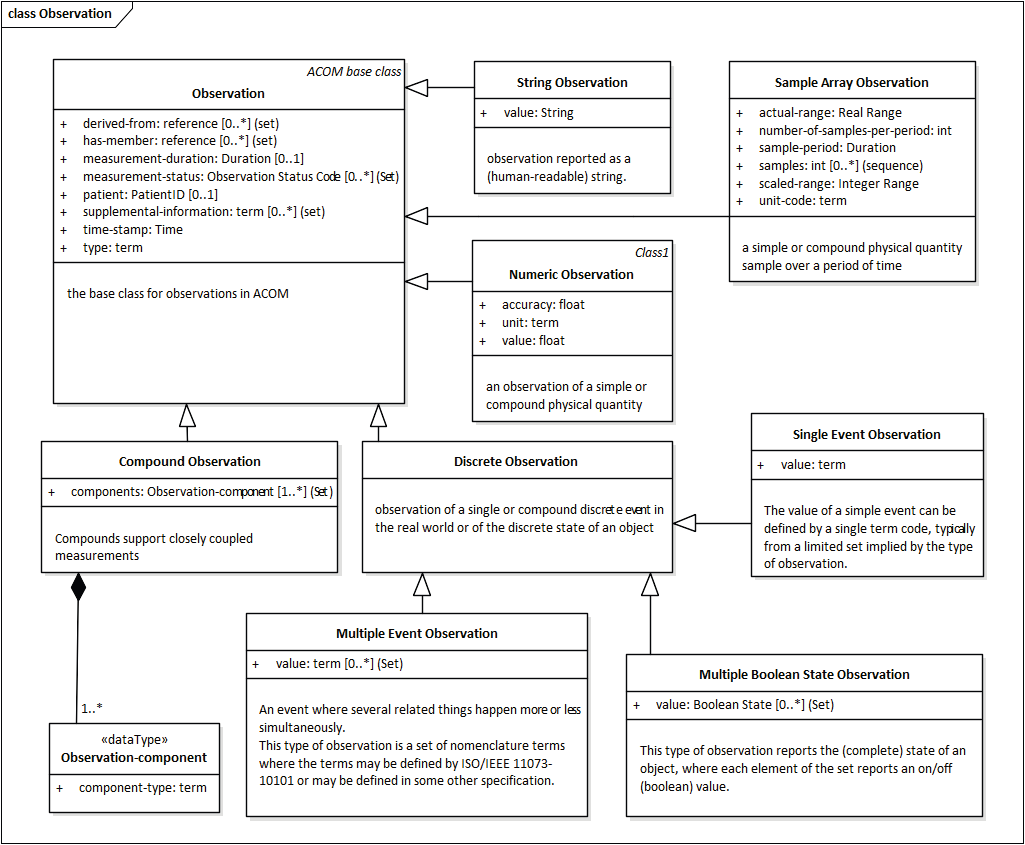
\includegraphics[width=1\textwidth]{figures/observation class.png}
            \caption{class Observation}
            \label{fig:observationClass}
        \end{figure}
        \begin{figure}[ht]
            \centering
            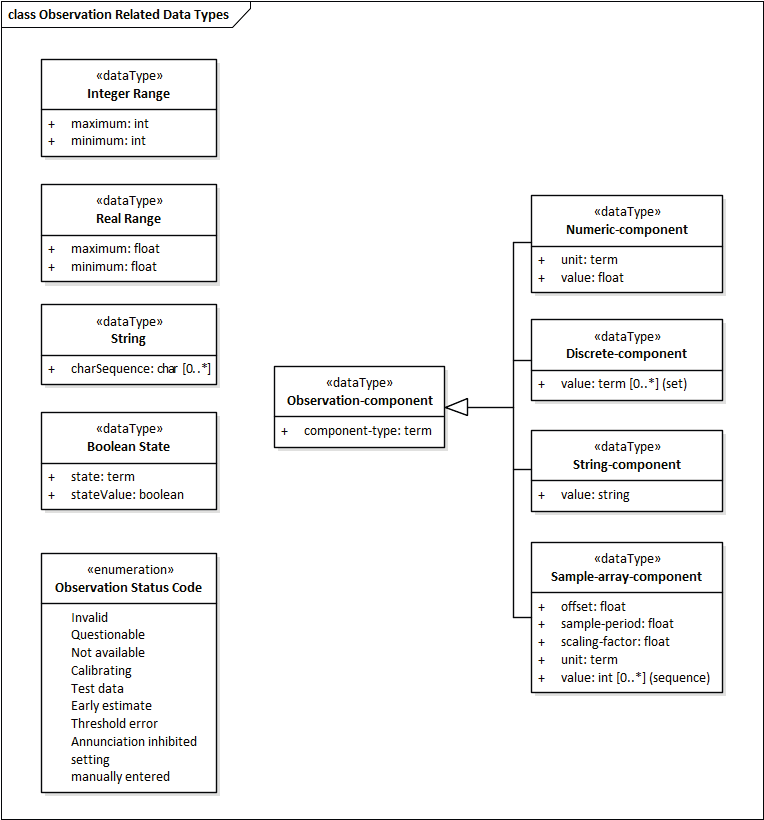
\includegraphics[width=1\textwidth]{figures/observation related data types class.png}
            \caption{class Observation Related Data Types}
            \label{fig:observationRelatedDataTypesClass}
        \end{figure}
        
    \section*{ACOM device specializations}
        Le specializzazioni dei dispositivi sono usate in questo standard per definire il contenuto informativo di uno specifico tipo di PHD.
        In parole povere sono classi che modellano alcuni tipi di PHD particolari (appartenenti alla classe IEEE 11073-104XX), di conseguenza contengono al loro interno le informazioni basiche sulla struttura del PHD (Power, Clock e SystemInfo), 
        un oggetto che modella il PHD e un oggetto Observation che modella le osservazioni. 
        Dato che il capitolo 8 del PDF su ACOM tratta tutti i tipi di PHD, userò il primo (un termometro), come esempio per gli altri.
        \newpage
        \subsection*{IEEE 11073-10408 thermometer}
        \begin{figure}[ht]
            \centering
            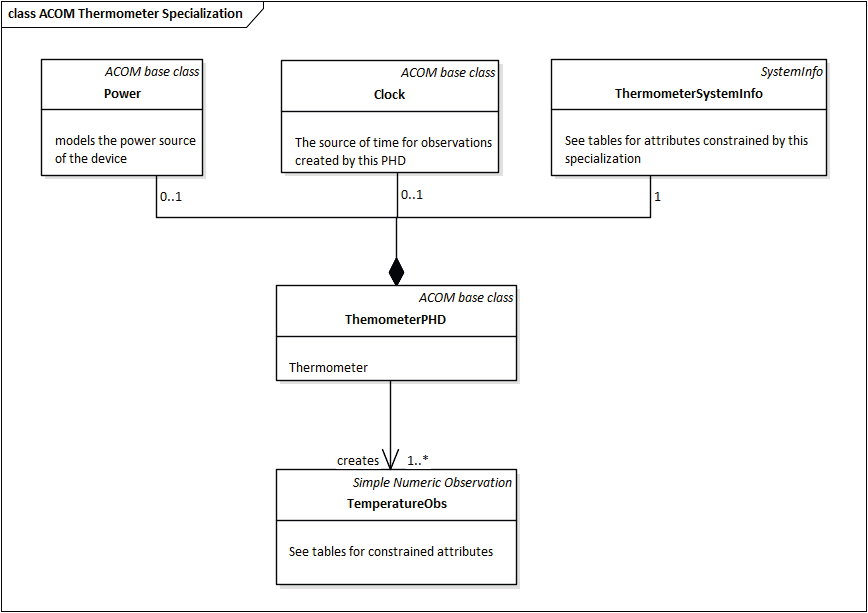
\includegraphics[width=1\textwidth]{figures/ACOM thermometer specialization class.png}
            \caption{class ACOM Thermometer Specialization}
        \end{figure}
\end{document}